\documentclass{beamer}

\usepackage{../../../latex_style/beamerthemeExecushares}
\usepackage{../../../latex_style/notations}

\title{Session 11: Optimality conditions}
\subtitle{Optimization and Computational Linear Algebra for Data Science}
\author{Léo Miolane}
\date{}

\setcounter{showSlideNumbers}{1}

\begin{document}
\setcounter{showProgressBar}{0}
\setcounter{showSlideNumbers}{0}

\frame{\titlepage}
\setcounter{framenumber}{0}
%\setcounter{showProgressBar}{1}
\setcounter{showSlideNumbers}{1}

\begin{frame}
	\frametitle{Contents}
	\begin{enumerate}
		\item Unconstrained optimization
		\item Constrained optimization and Lagrange multipliers
		\item Convex constrained optimization problems
	\end{enumerate}
\end{frame}

\section{Unconstrained optimization}
\begin{frame}[t]{Questions about the video?}
	\grid

	\vspace{-0.2cm}
	\begin{itemize}
		\item Global minimizer $\implies$ local minimizer $\implies$ critical point.
		\item Critical point + positive definite Hessian $\implies$ local minimizer.
	\end{itemize}

\end{frame}

\begin{frame}[t]{Hessian at a critical point}
	%\grid

	\vspace{-1.6cm}
	\begin{columns}
		\begin{column}{0.7\textwidth}
			\hspace*{-1.7cm}
			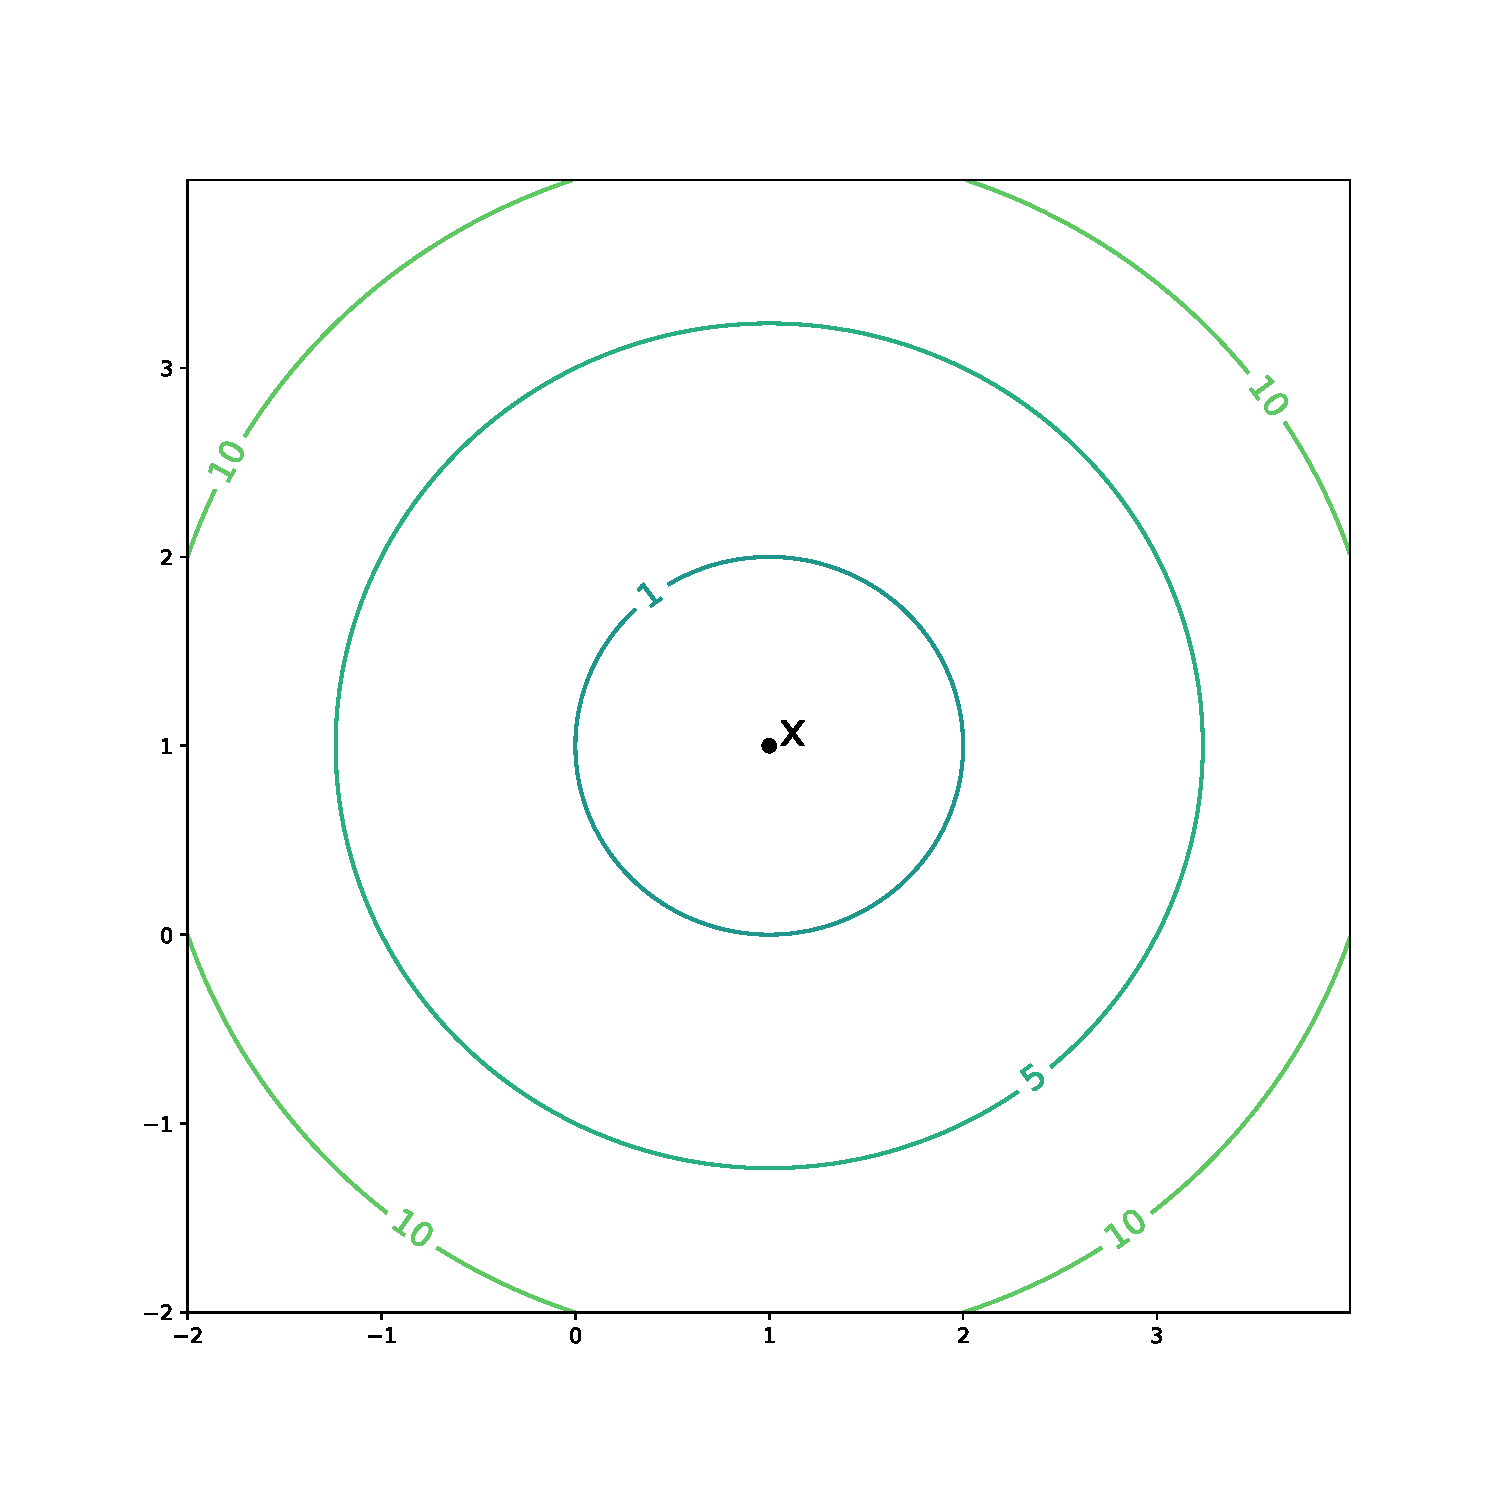
\includegraphics[width=11.0cm]{contour_min1.pdf}
		\end{column}
		\hspace*{0.2cm}
		\begin{column}{0.29\textwidth}
			The eigenvalues of the Hessian at $x$ are
			\begin{enumerate}
				\item $
					\begin{cases}
						\lambda_1 = 1 \\
						\lambda_2 = -1
					\end{cases}
					$
				\item $
					\begin{cases}
						\lambda_1 = 1 \\
						\lambda_2 = 1
					\end{cases}
					$
				\item $
					\begin{cases}
						\lambda_1 = 2 \\
						\lambda_2 = 1
					\end{cases}
					$
				\item $
					\begin{cases}
						\lambda_1 = -1 \\
						\lambda_2 = -1
					\end{cases}
					$
			\end{enumerate}
		\end{column}
	\end{columns}

\end{frame}
\begin{frame}[t]{Hessian at a critical point}
	%\grid

	\vspace{-1.6cm}
	\begin{columns}
		\begin{column}{0.7\textwidth}
			\hspace*{-1.7cm}
			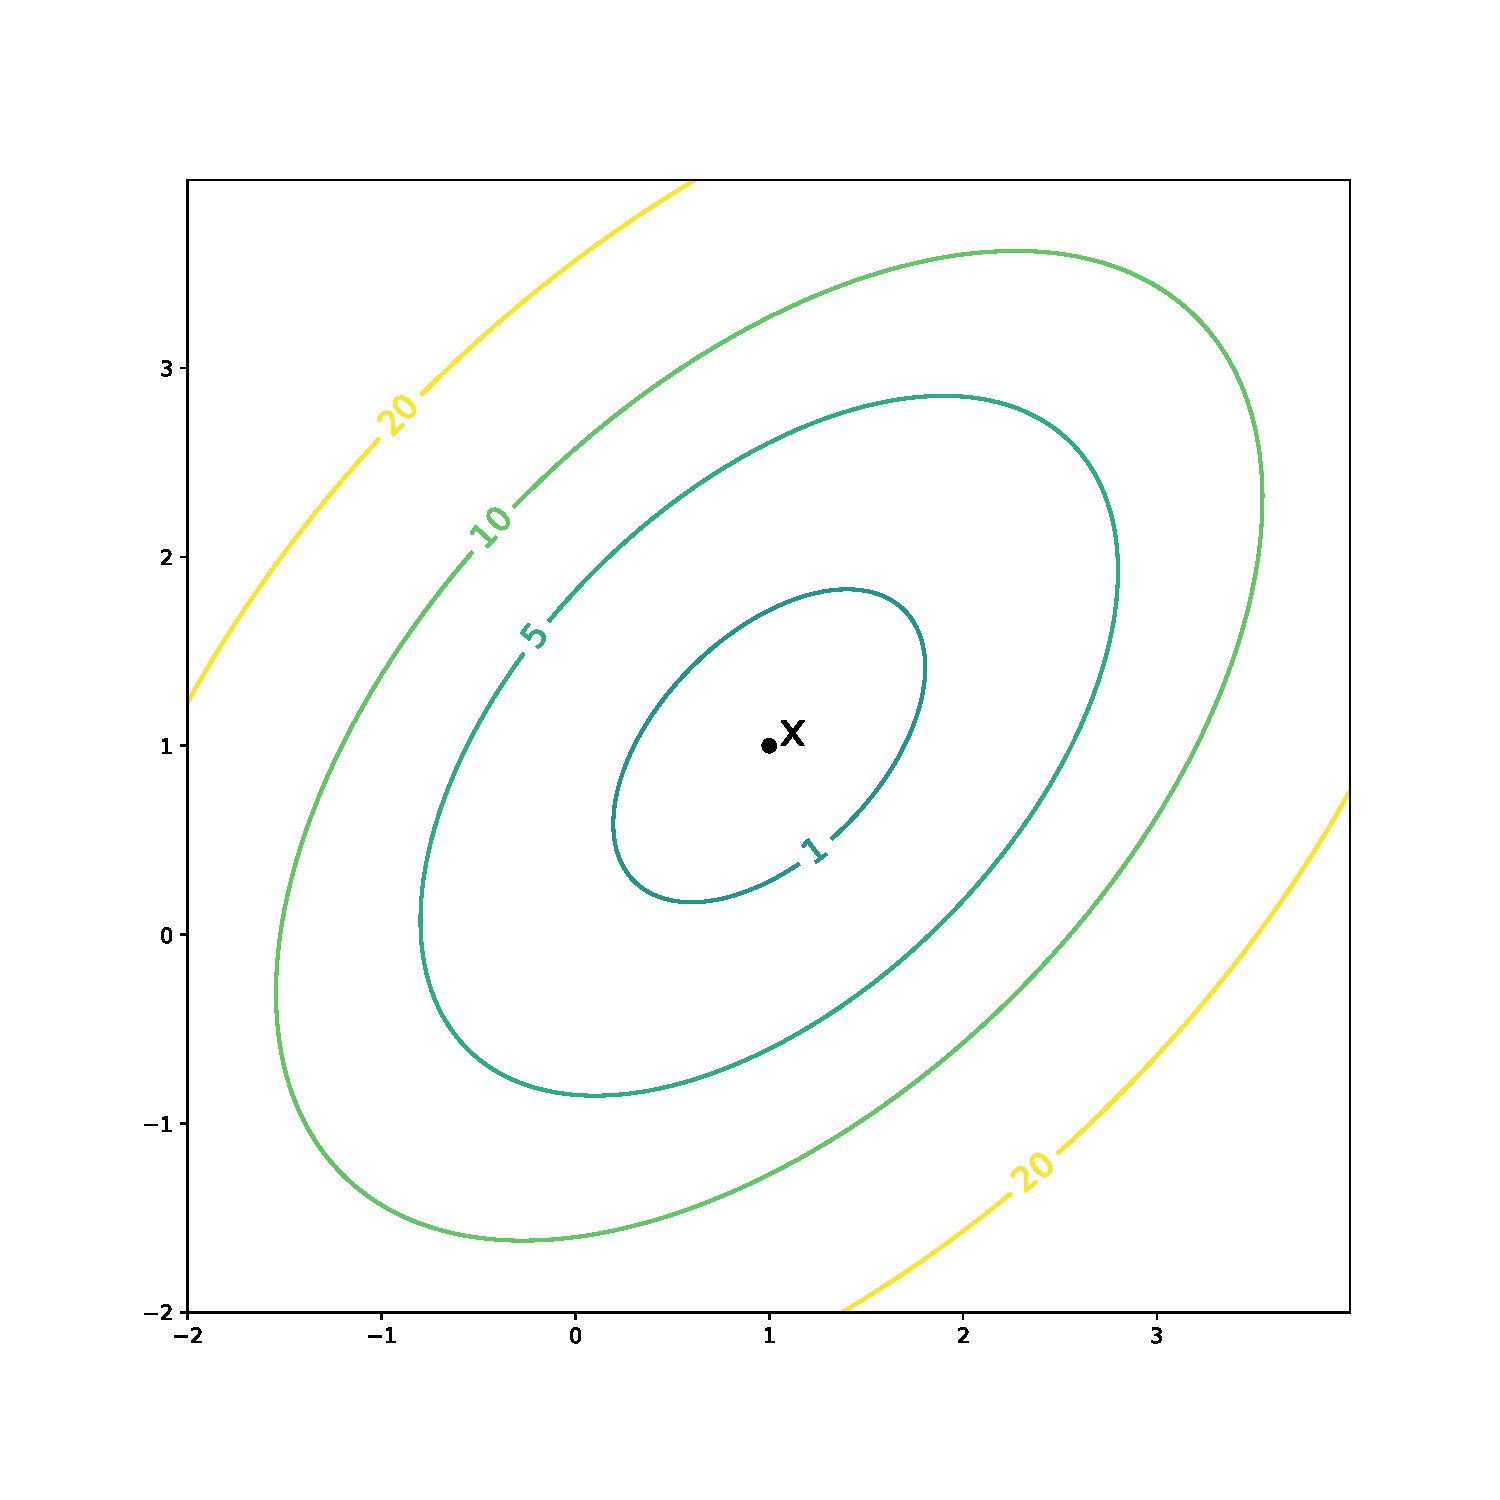
\includegraphics[width=11.0cm]{contour_min2.pdf}
		\end{column}
		\hspace*{0.2cm}
		\begin{column}{0.29\textwidth}
			The eigenvalues of the Hessian at $x$ are
			\begin{enumerate}
				\item $
					\begin{cases}
						\lambda_1 = 1 \\
						\lambda_2 = -3
					\end{cases}
					$
				\item $
					\begin{cases}
						\lambda_1 = 2 \\
						\lambda_2 = 2
					\end{cases}
					$
				\item $
					\begin{cases}
						\lambda_1 = 1 \\
						\lambda_2 = 3
					\end{cases}
					$
				\item $
					\begin{cases}
						\lambda_1 = -1 \\
						\lambda_2 = -1
					\end{cases}
					$
			\end{enumerate}
		\end{column}
	\end{columns}

\end{frame}
\begin{frame}[t]{Hessian at a critical point}
	%\grid

	\vspace{-1.6cm}
	\begin{columns}
		\begin{column}{0.7\textwidth}
			\hspace*{-1.7cm}
			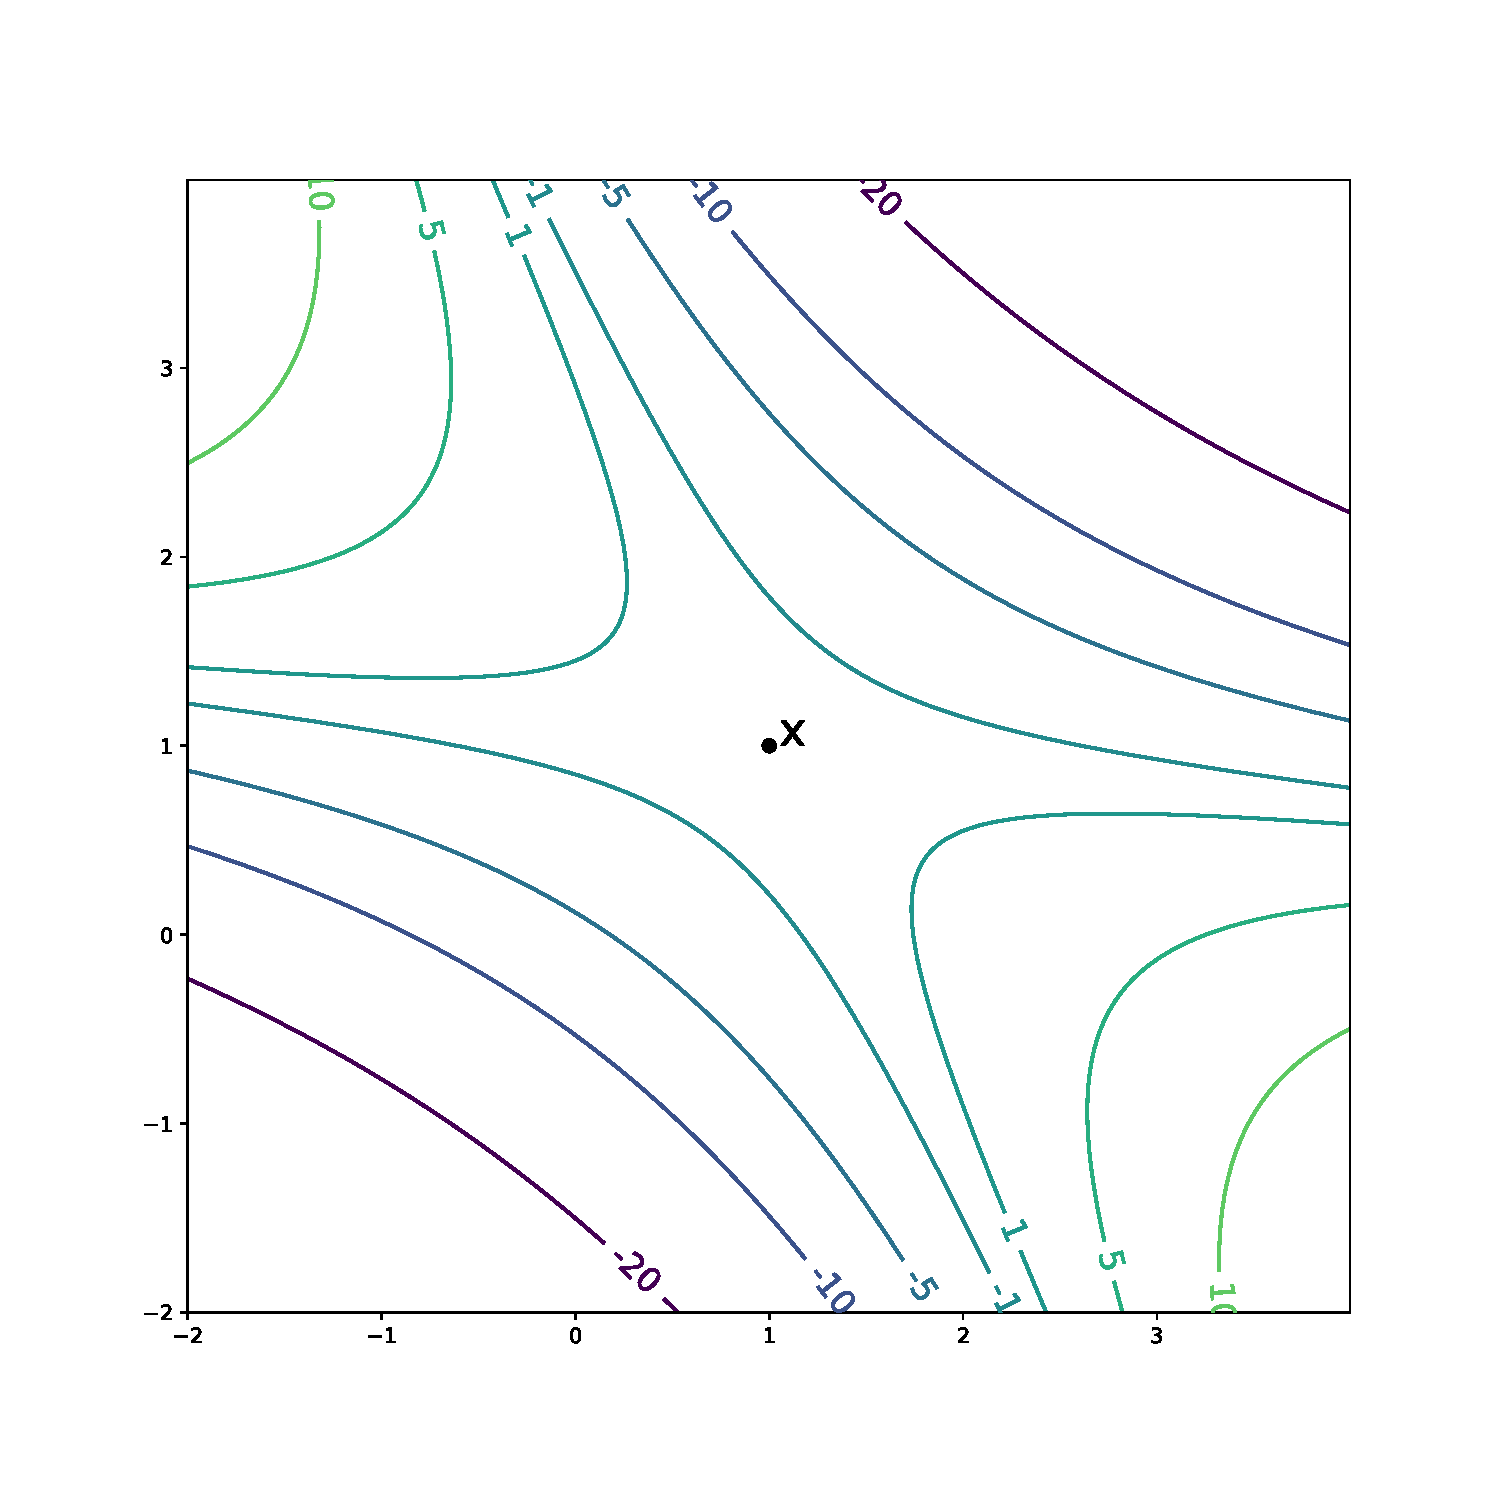
\includegraphics[width=11.0cm]{contour_saddle.pdf}
		\end{column}
		\hspace*{0.2cm}
		\begin{column}{0.29\textwidth}
			The eigenvalues of the Hessian at $x$ are
			\begin{enumerate}
				\item $
					\begin{cases}
						\lambda_1 = 1 \\
						\lambda_2 = -3
					\end{cases}
					$
				\item $
					\begin{cases}
						\lambda_1 = 2 \\
						\lambda_2 = 2
					\end{cases}
					$
				\item $
					\begin{cases}
						\lambda_1 = 1 \\
						\lambda_2 = 3
					\end{cases}
					$
				\item $
					\begin{cases}
						\lambda_1 = -1 \\
						\lambda_2 = -1
					\end{cases}
					$
			\end{enumerate}
		\end{column}
	\end{columns}

\end{frame}

\section{Constrained optimization}

\begin{frame}[t]{General formulation}
	\grid

	Constrained optimization problems take the form:
	$$
	\begin{array}{lll}
		\text{minimize} & f(x) & \\
		\text{subject to} & g_i(x) \leq 0, & i=1, \dots, m \\
						  & h_i(x) = 0, & i=1, \dots, p,
	\end{array}
	$$
	with variable $x \in \R^n$.
\end{frame}

\begin{frame}[t]{Feasible points}
	\grid
	\begin{definition}
		A point $x \in \R^n$ is \emph{feasible} if it satisfies all the constraints: $g_1(x) \leq 0, \dots, g_m(x)\leq  0$ and $h_1(x) = 0, \dots, h_p(x) = 0$. 
	\end{definition}


\end{frame}

\begin{frame}[t]{Question}
	\grid

	If $x$ is a solution to
	$$
	\begin{array}{lll}
		\text{minimize} & f(x) & \\
		\text{subject to} & g_i(x) \leq 0, & i=1, \dots, m \\
						  & h_i(x) = 0, & i=1, \dots, p,
	\end{array}
	$$
	do we have $\nabla f(x) = 0$ ?
\end{frame}


\begin{frame}[t]{First order optimality condition}
	\grid

	\pause
	\pause
	\pause
\end{frame}

\begin{frame}[t]{First order optimality condition}
	\grid

	\vspace{-0.4cm}
	\begin{block}{Theorem}
		If $x$ is a solution and if $\nabla h_1(x), \dots, \nabla h_p(x), \{\nabla g_i(x) \, | \, g_i(x) = 0 \}$ are linearly independent,
		then there exists $\lambda_1, \dots, \lambda_m \geq 0$ and $\nu_1, \dots, \nu_p \in \R$ such that:
		$$
		\nabla f(x) \ + \ \sum_{i=1}^m \lambda_i \nabla g_i(x) \ + \ \sum_{i=1}^p \nu_i \nabla h_i(x)  \ = \ 0.
		$$
		Moreover, for all  $i\in \{1, \dots, m\}$, if $g_i(x) < 0$ then $\lambda_i = 0$.
	\end{block}

\end{frame}

\begin{frame}[t]{Example}
	\grid

	\vspace{-0.2cm}
	Let $u \in \R^n$ be a non-zero vector. \quad
	$
	\begin{array}{lll}
		\text{Minimize} & \langle x,u \rangle & \\
		\text{subject to} & \|x\|^2 = 1.
	\end{array}
	$
	\pause
\end{frame}


\section{Convex constrained optimization}


\begin{frame}[t]{General formulation}
	\grid

	We say that the constrained optimization problem
	$$
		\begin{array}{lll}
			\text{minimize} & f(x) & \\
			\text{subject to} & g_i(x) \leq 0, & i=1, \dots, m \\
							  & h_i(x) = 0, & i=1, \dots, p,
		\end{array}
		$$
	is convex when $f$, $g_1, \dots, g_m$ are convex and $h_1, \dots, h_p$ are affine.
\end{frame}

\begin{frame}[t]{Karush-Kuhn-Tucker Theorem}
	\grid

	\vspace{-0.4cm}
	\begin{block}{Theorem (KKT)}
		Assume that the problem is convex and that there exists a feasible point $x_0$ such that $g_i(x_0) < 0$ for all $i$.

		Then $x$ is a solution if and only if $x$ is feasible and there exists $\lambda_1, \dots, \lambda_m \geq 0$, $\nu_1, \dots, \nu_p \in \R$ such that:
		$$
		\begin{cases}
			\displaystyle
			\nabla f(x) \ + \ \sum_{i=1}^m \lambda_i \nabla g_i(x) \ + \ \sum_{i=1}^p \nu_i \nabla h_i(x)  \ = \ 0. \\
			\lambda_i g_i(x) = 0, \ \ \text{for all} \ \ i \in \{1, \dots, p\}.
		\end{cases}
		$$
		\vspace{-0.3cm}
	\end{block}

\end{frame}
\begin{frame}[t]{Example: Ridge regression}
	\grid
	$$
		\begin{array}{lll}
			\text{minimize} & \|Ax-y\|^2 & \\
			\text{subject to} & \|x\|^2 \leq r^2.
		\end{array}
		$$
	 
		\pause
\end{frame}

\begin{frame}[t]{Example}
	\grid

	\vspace{-0.2cm}
	\only<1>{
	Let $u,v \in \R^n$ such that $\|v\|=1$. Solve:
	$$
		\begin{array}{lll}
			\text{minimize} & \|x-u\|^2 & \\
			\text{subject to} & x \perp v.
		\end{array}
		$$
	}

	\pause


\end{frame}

\appendix
\backupbegin
\begin{frame}[t]
	\frametitle{Questions?}
	\grid

	\pause
\end{frame}
\backupend




\end{document}
